\documentclass[border=3pt,tikz]{standalone}
\usepackage{amsmath,amssymb}
\usepackage{bm} % math bold
\usepackage[outline]{contour} % glow around text
\contourlength{1.2pt}

\usepackage{tikz}
\usetikzlibrary{patterns}
\tikzset{>=latex}

\begin{document}

% NUMERICAL SOLUTIONS
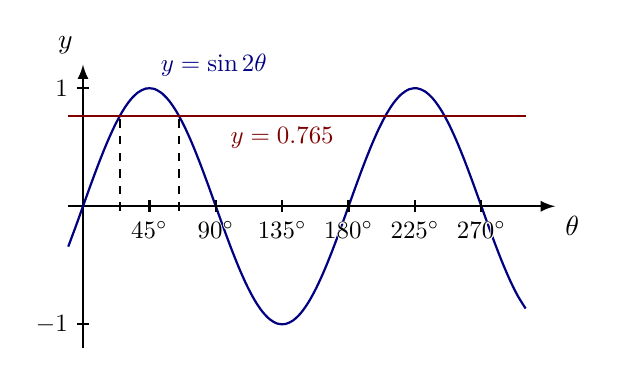
\begin{tikzpicture}[scale=1.5,xscale=1/80]
  
  \def\N{60}
  \def\xmin{-10}  \def\xmax{320}
  \def\ymin{-1.2} \def\ymax{1.2}
  \def\tmin{-10}  \def\tmax{300}
  \def\blue{black!50!blue}, \def\red{black!50!red}
  \def\value{0.765}
  \def\Dtheta{20}
  
  % axes
  \draw[->,thick]
    (\xmin,0) -- (\xmax,0)
    node[anchor=north west] {$\theta$};
  \draw[->,thick]
    (0,\ymin) -- (0,\ymax)
    node[anchor=south east] {$y$};
  
  % plots
  \draw[thick,\blue,variable=\t,domain=\tmin:\tmax,samples=\N,smooth]
    plot (\t,{sin(2*\t)});
  \draw[thick,\red,variable=\t,domain=\tmin:\tmax,samples=\N,smooth]
    plot (\t,\value);
  
  % function labels
  \node[\blue,above right=1pt,scale=0.9] at (45,1) {$y=\sin2\theta$};
  \node[\red, below=1pt,scale=0.9] at (135,\value) {$y=\value$};
  
  % numerical solutions
  \draw[dashed,thick] (45-\Dtheta,-\value*0.05) -- (45-\Dtheta,\value*1.05);
  \draw[dashed,thick] (45+\Dtheta,-\value*0.05) -- (45+\Dtheta,\value*1.05);
  
  % ticks
  \foreach \x in {45,90,135,180,225,270}{
    \draw[thick]
      (\x,0.05) -- (\x,-0.05) node[below,scale=0.9] {\contour{white}{$\x^\circ$}};}
  \foreach \y in {1,-1}{
    \draw[thick]
      (4,\y) -- (-4,\y) node[left,scale=0.9] {$\y$};}
   
\end{tikzpicture}

\end{document}